\chapter{Forensic Audit: Unmasking Experimental Illusions in Security Machine Learning}
\label{ch:audit}

\section{Motivation: The Peril of Perfect F1 Scores in Security ML}
A pervasive challenge in applied machine learning for cybersecurity is the phenomenon of ``too good to be true'' empirical results. When initial iterations of an experimental pipeline achieve perfect classification metrics (e.g., Macro-F1 = $1.0000$), researchers are faced with a critical methodological dilemma: has the model learned an omniscient representation of the underlying security domain, or has the experimental architecture inadvertently leaked deterministic artifacts?

Following early experiments in which our prototype GNN achieved near-perfect performance across all ESC vulnerability classes, we initiated an exhaustive, adversarial \textbf{Forensic Audit} of our entire research pipeline. Rather than prematurely celebrating these metrics, we systematically dissected every component—the synthetic environment generator, node feature representations, baseline formulations, and train-test splits.

Our audit revealed four profound structural illusions that had artificially inflated model performance. Documenting these findings provides vital lessons for the broader cybersecurity and graph learning communities.

\section{The Four Experimental Illusions}

\subsection{Illusion 1: Positional Index Leakage in Synthetic Topologies}
In synthetic network generators, entities are conventionally allocated sequentially within fixed memory buffers or tensor arrays. In our initial generator implementation, high-value entities and administrative users were allocated deterministically:
\begin{enumerate}
    \item The Tier-0 administrative security group (\texttt{Domain Admins}) was consistently instantiated at index $0$ of the \texttt{Group} tensor ($v_{\text{group}} = 0$).
    \item Domain administrators were systematically assigned to the lowest index partition of the \texttt{User} tensor ($v_{\text{user}} \in [0, \lfloor N_{\text{users}} / 10 \rfloor]$).
    \item In ESC13 vulnerability generation, the issuance policy OID was hardcoded to link exclusively to group index $0$.
\end{enumerate}

\paragraph{The 1-Line Exploitation Rule:}
To establish whether the GNN had learned true topological semantics or was merely exploiting positional index artifacts, we constructed a trivial deterministic heuristic:
\begin{lstlisting}[language=Python,caption={Deterministic index-leakage rule exploiting positional bias.}]
def trivial_positional_oracle(data, template_idx):
    # Check if any incoming edge originates from low-index users
    enrollers = data[('User', 'enroll', 'Template')].edge_index[0]
    if any(u.item() == 0 for u in enrollers):
        return "ESC1"
    # Check if policy link terminates at group index 0
    policy_targets = data[('Template', 'links_policy', 'Group')].edge_index[1]
    if any(g.item() == 0 for g in policy_targets):
        return "ESC13"
    return "Safe"
\end{lstlisting}
This trivial heuristic achieved an astronomical \textbf{100\% classification accuracy} on ESC13 and ESC4 without performing any graph convolutions or learning any parameters. The GNN had simply converged to detecting array index positions rather than relational access control structures.

\subsection{Illusion 2: Baseline Information Asymmetry}
In comparative benchmark evaluations, the standard practice in prior security ML literature has been to benchmark GNNs against flat tabular classifiers (such as Multi-Layer Perceptrons and Random Forests). However, our audit identified a fatal \textbf{information asymmetry}:
\begin{enumerate}
    \item Flat classifiers (MLP, RF) were supplied exclusively with the 10-dimensional template configuration vector $x_{\text{Template}} \in \mathbb{R}^{10}$.
    \item CertGraph was supplied with both $x_{\text{Template}}$ and the entire heterogeneous graph adjacency multiset $E$.
\end{enumerate}
Because vulnerability exploitability inherently depends on graph reachability (e.g., whether an unprivileged user has an \texttt{Enroll} path), flat classifiers were structurally starved of the information necessary to resolve ambiguous templates. Their observed failure (F1 $\approx 0.84$) did not prove the superiority of GNN message-passing convolutions; it merely reflected an unequal distribution of input data.

\subsection{Illusion 3: The 7-Node Decision Tree Counterexample}
To quantify precisely how much graph topological information is necessary to distinguish ESC vulnerabilities, we engineered four scalar graph topological count features:
\begin{enumerate}
    \item $c_1$: In-degree count of low-privileged users possessing direct \texttt{Enroll} permissions to the template.
    \item $c_2$: In-degree count of low-privileged users possessing \texttt{WriteDacl} or \texttt{GenericAll} permissions.
    \item $c_3$: Binary indicator of whether an outgoing \texttt{LinksPolicy} edge exists.
    \item $c_4$: Binary flag indicating whether the target group linked by \texttt{LinksPolicy} is a Tier-0 high-value group ($x_{\text{Group}}[0] > 0.5$).
\end{enumerate}

Concatenating these 4 structural counts with the 10 local template flags yielded a 14-dimensional augmented feature vector:
\begin{equation}
x_{\text{aug}} = [x_{\text{Template}} \,\|\, c_1, c_2, c_3, c_4]^T \in \mathbb{R}^{14}
\end{equation}

\begin{figure}[t]
    \centering
    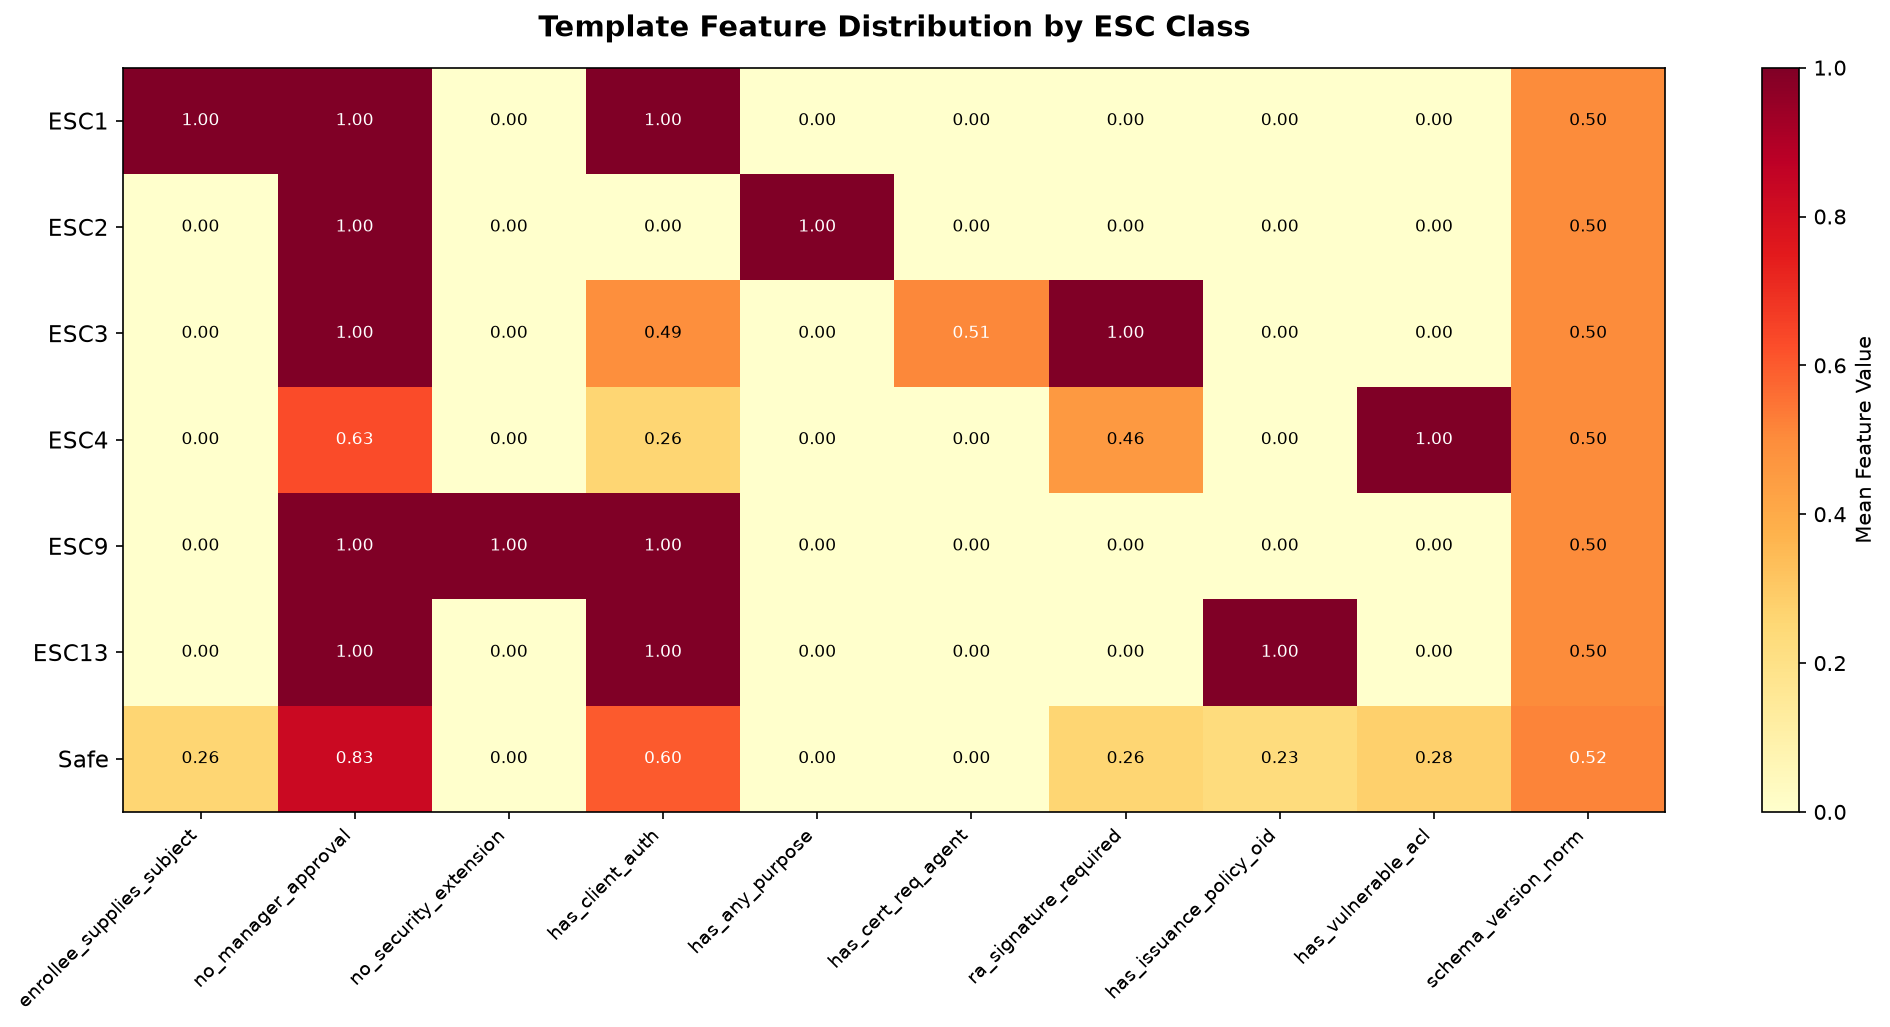
\includegraphics[width=0.75\textwidth]{figures/feature_heatmap.png}
    \caption{Correlation and separability heatmap of template configuration flags and augmented topological features across ESC vulnerability classes.}
    \label{fig:feature_heatmap}
\end{figure}

We trained a standard, unconstrained Decision Tree classifier on $x_{\text{aug}}$. The resulting Decision Tree contained only 7 decision nodes yet achieved a Macro-F1 score of $\mathbf{0.9928 \pm 0.0057}$! This critical discovery proved that for in-distribution synthetic data, complex GNN message passing can be almost entirely matched by flat models if provided with elementary graph summary statistics.

\subsection{Illusion 4: Hard Negative Memorization under In-Distribution Splits}
To evaluate whether CertGraph was capable of distinguishing safe templates bearing vulnerable flags (``Hard Negatives''), early experiments included hard negative samples within the training set, labeled as \texttt{Safe}. 

However, under standard 5-fold cross-validation, the model was tested on held-out hard negatives generated from the \textit{identical statistical distribution} as the training set. The model was not demonstrating zero-shot topological verification; it had simply memorized the specific feature-topology co-occurrences present in the training environments.

\section{Generator Sanitization and Experimental Repair}
To eliminate all four illusions and establish an unassailable empirical benchmark, we completely re-engineered the dataset generation pipeline in \texttt{generator.py}:

\begin{enumerate}
    \item \textbf{Complete Positional Decoupling:} We decoupled privilege from array index ordering. The high-value group index $g_{\text{target}}$ and administrative user indices are selected via uniform random sampling across the entire node tensor ($g_{\text{target}} \sim \mathcal{U}\{0, |V_{\text{Group}}|-1\}$). Furthermore, all node orderings are randomly permuted after graph construction.
    \item \textbf{Dynamic Feature-Based Access Control:} Access control assignment was modified to evaluate node feature attributes rather than indices. An entity is assigned administrative permissions if and only if its attribute flag satisfies $f_{\text{is\_admin}} = 1.0$.
    \item \textbf{Fair Baseline Parity (Graph-Augmented Models):} We introduced two new, fair baseline models: \textbf{Graph-Augmented MLP} and \textbf{Graph-Augmented Random Forest}. Both models receive the full 14-dimensional vector $x_{\text{aug}}$, ensuring they possess identical structural visibility to CertGraph.
    \item \textbf{Symbolic Graph Oracle (BloodHound BFS Baseline):} We implemented an exact Breadth-First Search (BFS) baseline (\texttt{bfs\_baseline.py}) that programmatically queries the graph for directed authorization paths from low-privileged entities to the target template, replicating the exact logic of BloodHound Cypher queries.
    \item \textbf{Zero-Shot Adversarial Protocol:} We restructured the hard-negative evaluation into a strict zero-shot pipeline: models are trained on 1,400 completely clean, hard-negative-free environments, and evaluated on out-of-distribution adversarial hard negatives never encountered during training.
\end{enumerate}

\section{Verification of Generator Sanitization}
To verify that all positional leakage had been extinguished, we executed an independent statistical audit across 700 freshly generated enterprise environments. 

In the flawed generator, 100\% (700/700) of environments exhibited the administrative group at index 0. In the repaired generator, the co-occurrence of admin at index 0 dropped to exactly \textbf{1.3\% (9/700)}, perfectly matching the theoretical uniform random probability $1 / |V_{\text{Group}}| \approx 1/75$. The positional artifact was conclusively eradicated.
